\documentclass{standalone}
\usepackage{standalone}

\begin{document}
\subsection{Suffix Trie}
Before knowing about Suffix Trie we should have a quick glance at Trie. Sometimes it is considered that the word "Trie" comes from the word "Retrieval". As generally Trie is used for storing string type of data or information and then retrieve. Trie is also known as digital tree, radix tree or prefix tree.
By formal definition a Trie is a tree containing a collection of strings with a single node per common prefix. It is the smallest tree such that:
\begin{enumerate}
	\item Every edge is labeled with a character {\bf \emph{C}} from the alphabet set of the whole string.
	\item Every node has at most one edge emanating from that node labeled as {\bf \emph{C}}.
	\item Every prefix of the string stored can be found along some path starting from the root of the tree.  
\end{enumerate}
Suffix Trie is nothing but only a Trie containing all the suffixes of a text {\bf \emph{T}}. Let's take a text {\bf \emph{T}} = "ATATACA".
All suffixes of the above text would be figure \ref{fig:suff}

\begin{figure}
	\centering
	\begin{BVerbatim}[fontsize=\Large]
	ATATACA
	 TATACA
	  ATACA
	   TACA
	    ACA
	     CA
	      A	
	\end{BVerbatim}
	\caption{Suffixes of the text "ATATACA".}
	\label{fig:suff}
\end{figure}
Now have to just build a Trie for all the suffixes. At first we need to add a special terminal character \$ to the end of the {\bf \emph{T}}. This is because
\begin{enumerate}
	\item \$ is a character that does not appear anywhere in {\bf \emph{T}} except at last and we define it as to be less than other characters. (For DNA sequences {\bf \emph{\$}}<{\bf \emph{A}}<{\bf \emph{C}}<{\bf \emph{G}}<{\bf \emph{T}})
	\item As a result {\bf \emph{\$}} guarantees no suffix is a prefix of any other suffix.
\end{enumerate}
So the resulting suffixes of the text {\bf \emph{T\$}}  will be figure \ref{fig:sufft}
\begin{figure}
	\centering
	\begin{BVerbatim}[fontsize=\Large]
	ATATACA$
	 TATACA$
	  ATACA$
	   TACA$
	    ACA$
	     CA$
	      A$
	       $	
	\end{BVerbatim}
	\caption{Suffixes of the text "ATATACA\$".}
	\label{fig:sufft}
\end{figure} 
Now Building Trie for the above suffixes will result in such Trie Tree as in .
\begin{figure}
	\centering
	\tikzstyle{block} = [rectangle, draw, line width=0.5mm,
	text centered]
	\tikzstyle{line} = [draw, -latex']
	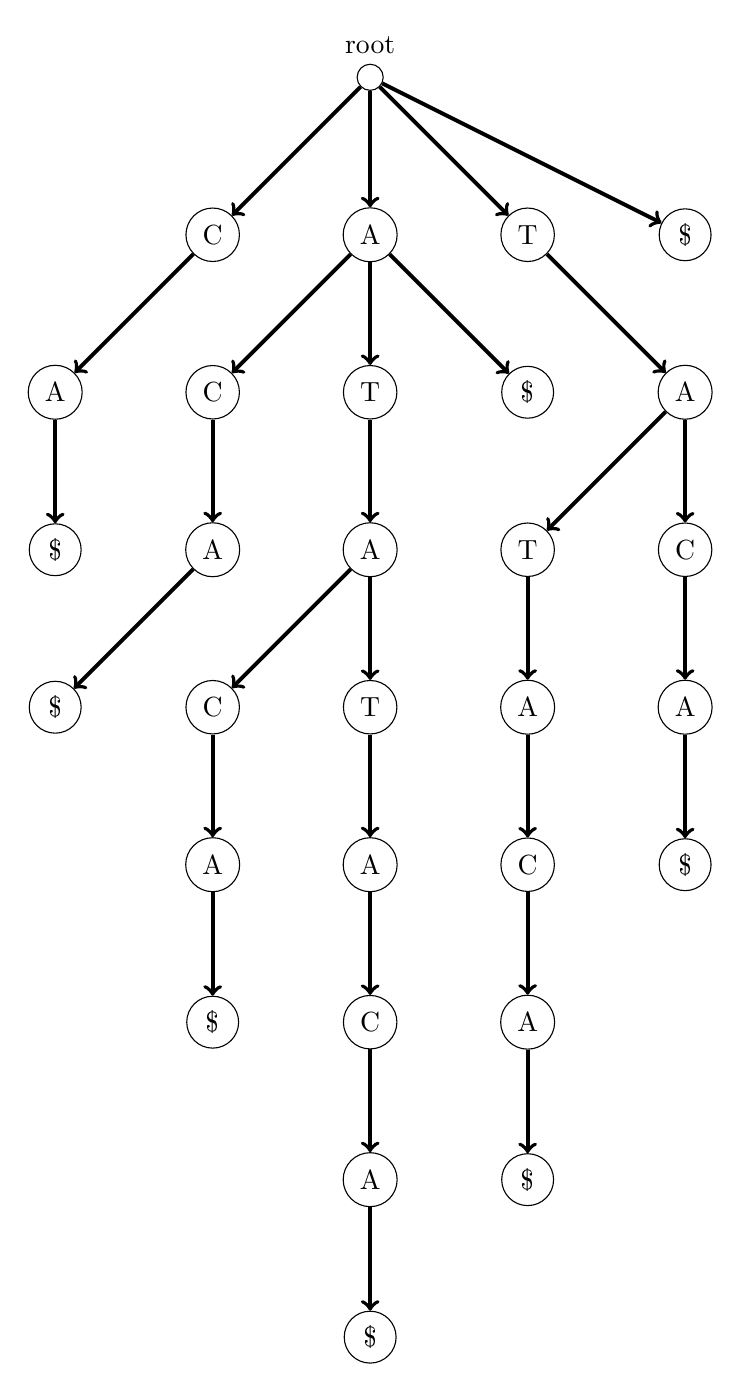
\begin{tikzpicture}[auto, node distance = 2cm]
	%level 1
	
	\node [circle, draw,label=root](lab) {};
	\node [circle, draw, below of=lab](lab1) {A};
	\draw [line width=0.5mm,->] (lab) -- (lab1);
	\node [circle, draw, left of=lab1](lab2) {C};
	\draw [line width=0.5mm,->] (lab) -- (lab2);
	\node [circle, draw, right of=lab1](lab3) {T};
	\draw [line width=0.5mm,->] (lab) -- (lab3);
	\node [circle, draw, right of=lab3](lab4) {\$};
	\draw [line width=0.5mm,->] (lab) -- (lab4);
	
	%level 2
	\node [circle, draw, below of=lab2](lab6) {C};
	\draw [line width=0.5mm,->] (lab1) -- (lab6);
	\node [circle, draw, left of=lab6](lab5) {A};
	\draw [line width=0.5mm,->] (lab2) -- (lab5);
	\node [circle, draw, right of=lab6](lab7) {T};
	\draw [line width=0.5mm,->] (lab1) -- (lab7);
	\node [circle, draw, right of=lab7](lab8) {\$};
	\draw [line width=0.5mm,->] (lab1) -- (lab8);
	\node [circle, draw, right of=lab8](lab9) {A};
	\draw [line width=0.5mm,->] (lab3) -- (lab9);
	
	%level 3
	\node [circle, draw, below of=lab5](lab10) {\$};
	\draw [line width=0.5mm,->] (lab5) -- (lab10);
	\node [circle, draw, right of=lab10](lab11) {A};
	\draw [line width=0.5mm,->] (lab6) -- (lab11);
	\node [circle, draw, right of=lab11](lab12) {A};
	\draw [line width=0.5mm,->] (lab7) -- (lab12);
	\node [circle, draw, right of=lab12](lab13) {T};
	\draw [line width=0.5mm,->] (lab9) -- (lab13);
	\node [circle, draw, right of=lab13](lab14) {C};
	\draw [line width=0.5mm,->] (lab9) -- (lab14);
	
	%level 4
	\node [circle, draw, below of=lab11](lab16) {C};
	\draw [line width=0.5mm,->] (lab12) -- (lab16);
	\node [circle, draw, left of=lab16](lab15) {\$};
	\draw [line width=0.5mm,->] (lab11) -- (lab15);
	\node [circle, draw, right of=lab16](lab17) {T};
	\draw [line width=0.5mm,->] (lab12) -- (lab17);
	\node [circle, draw, right of=lab17](lab18) {A};
	\draw [line width=0.5mm,->] (lab13) -- (lab18);
	\node [circle, draw, right of=lab18](lab19) {A};
	\draw [line width=0.5mm,->] (lab14) -- (lab19);
	
	%level 5
	\node [circle, draw, below of=lab16](lab20) {A};
	\draw [line width=0.5mm,->] (lab16) -- (lab20);
	\node [circle, draw, right of=lab20](lab21) {A};
	\draw [line width=0.5mm,->] (lab17) -- (lab21);
	\node [circle, draw, right of=lab21](lab22) {C};
	\draw [line width=0.5mm,->] (lab18) -- (lab22);
	\node [circle, draw, right of=lab22](lab23) {\$};
	\draw [line width=0.5mm,->] (lab19) -- (lab23);
	
	%level 6
	\node [circle, draw, below of=lab20](lab24) {\$};
	\draw [line width=0.5mm,->] (lab20) -- (lab24);
	\node [circle, draw, right of=lab24](lab25) {C};
	\draw [line width=0.5mm,->] (lab21) -- (lab25);
	\node [circle, draw, right of=lab25](lab26) {A};
	\draw [line width=0.5mm,->] (lab22) -- (lab26);

	%level 6
	\node [circle, draw, below of=lab25](lab27) {A};
	\draw [line width=0.5mm,->] (lab25) -- (lab27);
	\node [circle, draw, right of=lab27](lab28) {\$};
	\draw [line width=0.5mm,->] (lab26) -- (lab28);
	
	%level 7
	\node [circle, draw, below of=lab27](lab29) {\$};
	\draw [line width=0.5mm,->] (lab27) -- (lab29);
	\end{tikzpicture}
	\caption{Cyclic Left Shift of the First Character of  \textbf{S}. } \label{fig:buildST}
\end{figure}
\subsubsection{Complexity Analysis of Suffix Trie}
As Trie takes a huge memory depending on alphabet size and number of keys to be inserted. Suffix Trie also takes such memory and complexity. Insert and Search in Suffix Trie requires {\bf \emph{O(key\_length)}}. How ever the memory requirement of Suffix Trie is {\bf \emph{O(alphabet\_size*key\_length*N)}}. Where N is the number of keys in Suffix Trie. For a text of length {\bf \emph{m}}, N = m - 1.
\end{document}